\documentclass[11pt]{article}

\usepackage[margin=1in]{geometry}
\usepackage[T1]{fontenc}
\usepackage[utf8]{inputenc}
\usepackage{lmodern}
\usepackage{microtype}
\usepackage{amsmath,amssymb,mathtools}
\usepackage{hyperref}
\usepackage{graphicx}
\usepackage{subcaption}
\usepackage{float}
\hypersetup{hidelinks}

\title{}
\author{Shreyas Kalvankar}
\date{\today}

\begin{document}
\maketitle

\section{Frozen-kernel Fourier alignment and frozen versus evolving NTK on \(S^1\)}

We consider a one-hidden-layer ReLU network on the circle
\[
	S^1=\{x(\theta)=(\cos\theta,\sin\theta):\theta\in[0,2\pi)\},
\]
equipped with the uniform probability measure
\[
	d\mu(\theta)=\frac{d\theta}{2\pi}.
\]
Let \(f^\star\in L^2(S^1,\mu)\) be the target function and let
\[
	f_m(\theta;\Theta)=\frac{1}{\sqrt m}\sum_{r=1}^m a_r\,\sigma(w_r^\top x(\theta)+b_r),
	\qquad
	\sigma(z)=\max\{z,0\},
\]
denote the network in NTK parameterization. Training is performed by gradient flow on the continuum least-squares loss
\[
	L(\Theta)=\frac12\int_0^{2\pi}\bigl(f_m(\theta;\Theta)-f^\star(\theta)\bigr)^2\,d\mu(\theta).
\]
If
\[
	r_t(\theta):=f_m(\theta;\Theta_t)-f^\star(\theta)
\]
is the residual, then the exact output dynamics gives
\[
	\partial_t r_t=-T_t r_t,
	\qquad
	(T_t g)(\theta)=\int_0^{2\pi}\Theta_t(\theta,\eta)g(\eta)\,d\mu(\eta),
\]
where \(\Theta_t(\theta,\eta)\) is the empirical time-dependent NTK. The frozen regime is obtained by fixing \(T_t\equiv T_0\), while the evolving regime keeps the full time dependence of \(T_t\).

On \(S^1\), the infinite-width reference operator \(T_\infty\) is convolutional and is diagonalized by the real Fourier basis
\[
	\phi_0(\theta)=1,\qquad
	\phi_{k,c}(\theta)=\sqrt2\cos(k\theta),\qquad
	\phi_{k,s}(\theta)=\sqrt2\sin(k\theta),\qquad k\ge 1.
\]
For each nonzero frequency \(k\), the corresponding ideal eigenspace is the two-dimensional Fourier plane
\[
	\mathcal F_k=\operatorname{span}\{\phi_{k,c},\phi_{k,s}\}.
\]
This is the basic reason that the eigenspace comparison must be done at the level of \emph{subspaces} rather than individual eigenvectors: even if the empirical kernel has recovered the correct frequency block perfectly, its numerical eigendecomposition may return any orthonormal basis inside this two-dimensional plane.

To study the low-mode dynamics, we project the exact ODE onto
\[
	H_K=\operatorname{span}\{\phi_0,\phi_{k,c},\phi_{k,s}:1\le k\le K\}.
\]
Let \(P_K\) be the orthogonal projection onto \(H_K\), and define
\[
	a_t:=P_K r_t\in H_K.
\]
Once the ordered Fourier basis
\[
	\Phi_K=(\phi_0,\phi_{1,c},\phi_{1,s},\dots,\phi_{K,c},\phi_{K,s})
\]
is fixed, the function \(a_t\) is equivalently represented by its coordinate vector
\[
	u_t\in\mathbb R^{2K+1}.
\]
Thus \(u_t\) is simply the vector of retained Fourier coefficients of the projected residual \(P_K r_t\). In these coordinates, the projected dynamics becomes
\[
	\dot u_t=-C_t^{(K)}u_t-\ell_t,
\]
where \(C_t^{(K)}=P_KT_tP_K\) is the compressed low-mode tangent operator written in the Fourier basis, and \(\ell_t\) is the leakage term produced by unresolved high modes. In the ideal infinite-width frozen theory,
\[
	C_t^{(K)}\to
	\Lambda_K=
	\operatorname{diag}(\lambda_0,\lambda_1,\lambda_1,\dots,\lambda_K,\lambda_K),
\]
so the dynamics is Fourier-diagonal. At finite width, the frozen branch replaces \(C_t^{(K)}\) by \(C_0^{(K)}\), while the evolving branch keeps the full time dependence of \(C_t^{(K)}\).

\subsection{Eigenspace alignment of the frozen empirical NTK with Fourier subspaces on \(S^1\)}
\label{subsec:frozen-ntk-eigenspace-alignment}

The frozen-kernel analysis asks how well the initial finite-width operator already reproduces the Fourier spectral structure of the infinite-width theory. For each \(k\ge 1\), let
\[
	U_k=[\phi_{k,c},\phi_{k,s}]
\]
be the orthonormal Fourier frame and let
\[
	V_k=[v_1,v_2]
\]
be an orthonormal basis of the corresponding empirical two-dimensional eigenspace of the frozen operator. The raw overlap matrix is
\[
	M_{\mathrm{raw}}=V_k^\top U_k.
\]
Each row of \(M_{\mathrm{raw}}\) gives the coordinates of one empirical eigenvector in the Fourier \((\cos,\sin)\)-plane. Thus each seed contributes the two points
\[
	(\langle v_1,\phi_{k,c}\rangle,\langle v_1,\phi_{k,s}\rangle),
	\qquad
	(\langle v_2,\phi_{k,c}\rangle,\langle v_2,\phi_{k,s}\rangle).
\]
These are the dots in the raw Fourier-plane plots. If a point lies near the unit circle, then the corresponding empirical vector lies mostly inside the Fourier plane \(\mathcal F_k\); if it lies well inside the unit disk, then part of that empirical vector leaks outside \(\mathcal F_k\). The raw plots therefore measure \emph{vector-wise overlap} with the Fourier block. However, they still contain the arbitrary rotation and sign ambiguity of the empirical basis inside its own two-dimensional plane, so spread around the circle does not by itself indicate poor subspace agreement.

A basis-free comparison is obtained through principal angles. If the singular values of \(V_k^\top U_k\) are
\[
	\sigma_1\ge \sigma_2,
\]
then the principal angles between the empirical eigenspace and the Fourier plane are
\[
	\theta_1=\arccos(\sigma_1),\qquad \theta_2=\arccos(\sigma_2).
\]
Two angles are needed because the subspaces are two-dimensional. The first angle measures whether there exists at least one direction in the empirical eigenspace that aligns well with the Fourier plane; the second measures whether the remaining orthogonal direction also aligns. Hence \(\theta_1\) small by itself indicates only \emph{partial} alignment, while both \(\theta_1\) and \(\theta_2\) small are needed to conclude that the full Fourier \(k\)-plane has been recovered.

A complementary basis-free quantity is the projector error
\[
	\|\widehat P_k-P_k\|_F,
\]
where \(P_k\) is the orthogonal projector onto \(\mathcal F_k\) and \(\widehat P_k\) is the orthogonal projector onto the empirical eigenspace. Unlike the raw coordinate plots, this error does not depend on the chosen basis inside the two-dimensional subspace.

The numerical results show a clear frequency-dependent hierarchy. At fixed width, low frequencies are much better aligned with the Fourier subspaces than high frequencies. The raw Fourier-plane coordinates at width \(256\) show that the clouds for \(k=1,\dots,5\) lie mostly near the unit circle, whereas for larger \(k\) they drift inward and become increasingly irregular. The mean shape plots tell the same story in function space: at width \(256\), the empirical components closely track the target Fourier shapes at the lowest frequencies, while phase shifts, amplitude distortions, and increased variability become more pronounced as \(k\) grows. The principal-angle curves confirm that both angles decrease with width for all displayed frequencies, but high-frequency blocks align much more slowly. By width \(1024\), the \(k=1\) and \(k=2\) subspaces are already very well aligned, \(k=3\) remains reasonably good, while \(k=5\) is only moderately aligned and \(k=10,15,20\) still have large second principal angles. The projector errors improve systematically with width at each fixed \(k\), but only the lowest frequencies fall clearly below the chosen tolerance threshold in the width range studied here.

An important point is that eigenvalue agreement alone is not sufficient. The absolute eigenvalue alignment error \(|\widehat\lambda_k-\lambda_k|\) and the empirical pair splitting \(|\widehat\lambda_{k,1}-\widehat\lambda_{k,2}|\) both decrease rapidly with width. However, these quantities can already be small in absolute value at high frequencies while the corresponding eigenspaces still exhibit poor subspace alignment, large principal angles, and large projector errors. Thus, for the frozen-kernel analysis, one must track the eigenspaces and not only the eigenvalues.

Taken together, these diagnostics show that the frozen empirical NTK becomes Fourier-organized progressively from low to high frequencies. At the widths considered here, the frozen kernel already provides an accurate low-frequency Fourier description for the first few modes, but this description deteriorates substantially as \(k\) increases. Therefore, the frozen frequency-by-frequency interpretation is justified for the lowest modes and only partially justified for intermediate ones; for higher frequencies it should be treated with caution. This is the correct baseline against which the evolving-kernel experiment must be compared.

\begin{figure}[H]
	\centering
	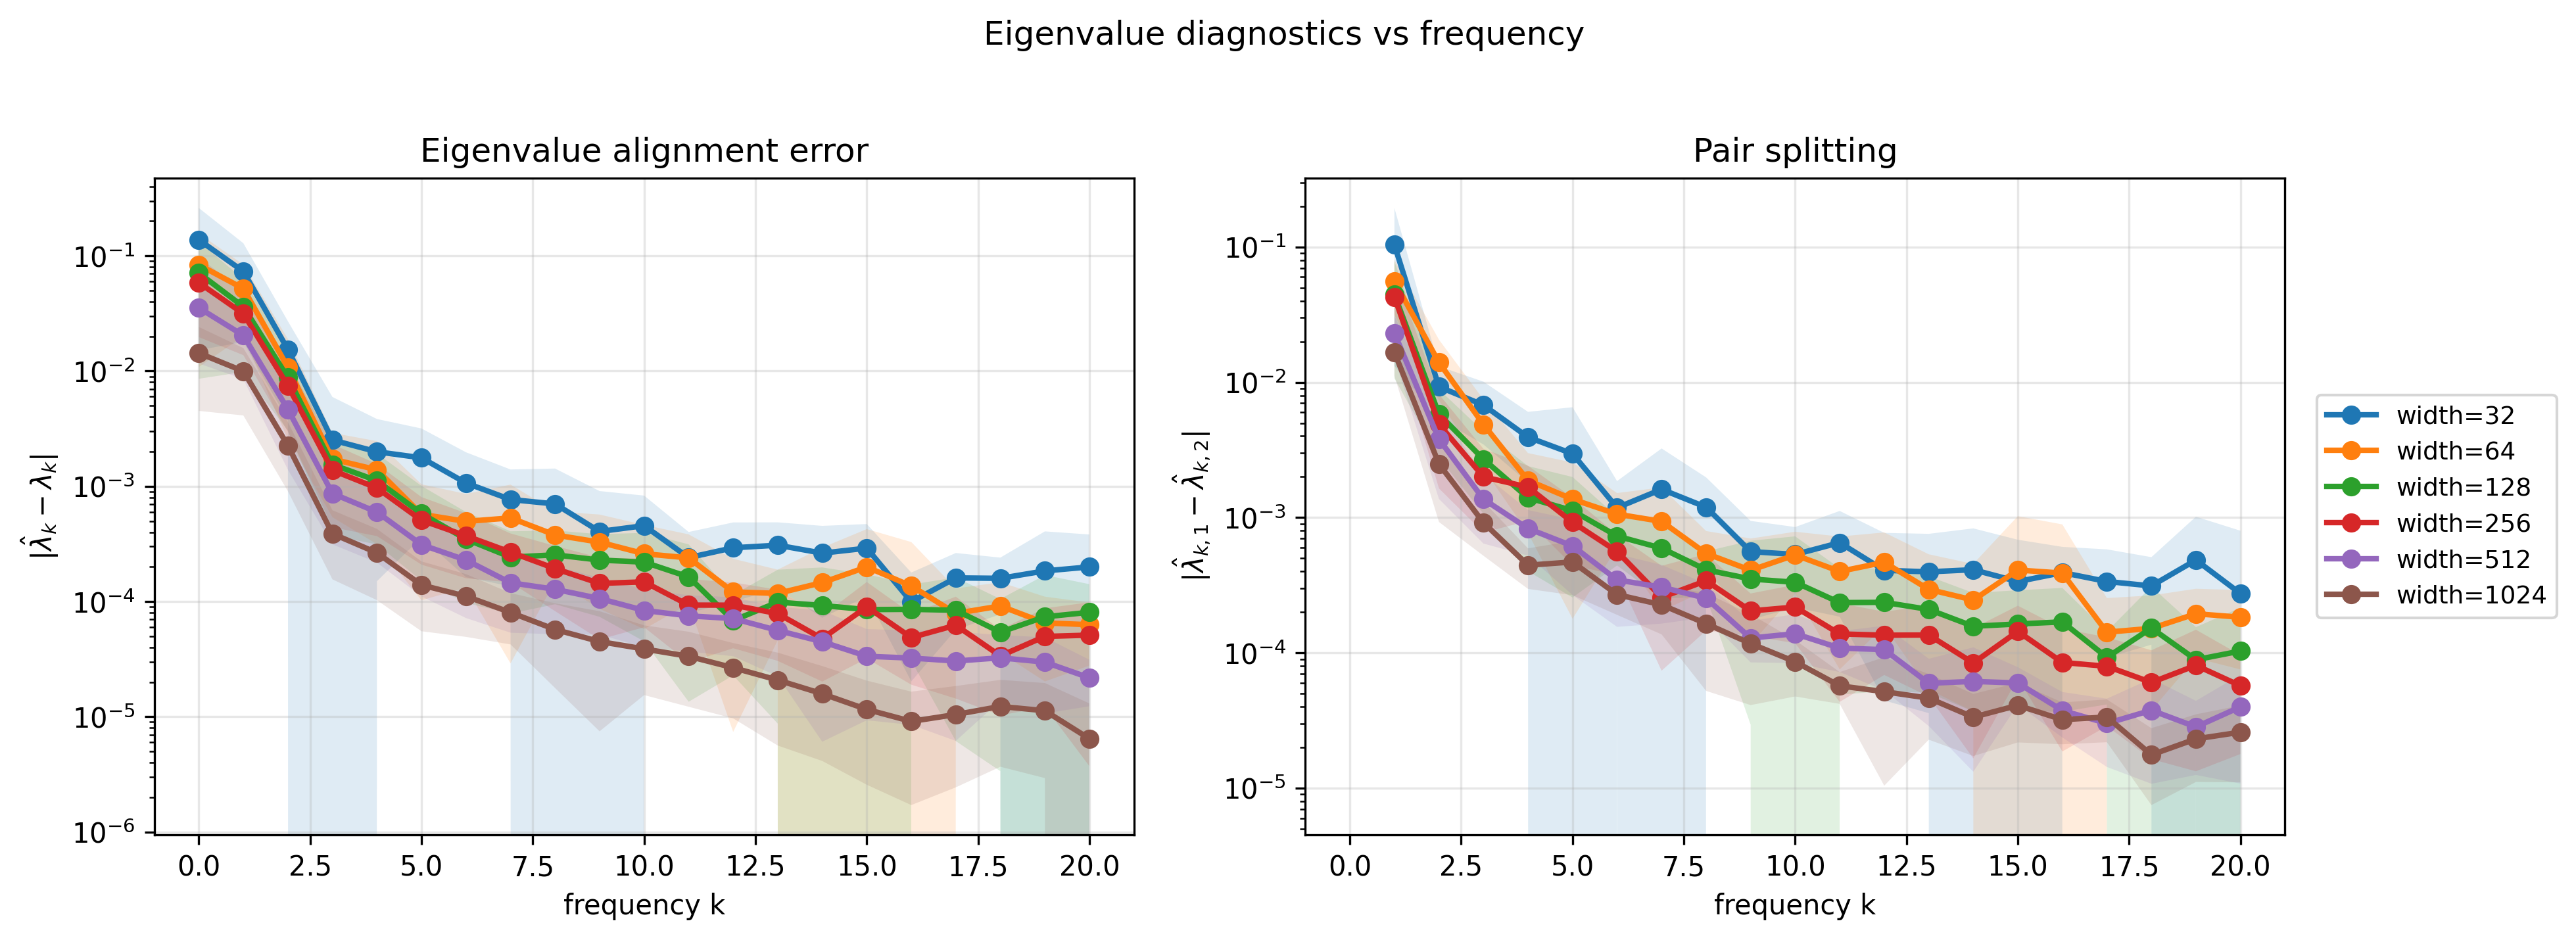
\includegraphics[width=0.92\textwidth]{images/ntk_eigenspace_alignment_on_S1/eigenvalue_error_vs_frequency.png}
	\caption{Eigenvalue diagnostics for the frozen empirical kernel as a function of frequency and width. Left: absolute eigenvalue alignment error \(|\widehat\lambda_k-\lambda_k|\). Right: empirical splitting of the two-dimensional \(k\)-pair, \(|\widehat\lambda_{k,1}-\widehat\lambda_{k,2}|\). Both quantities decrease rapidly with width, but small absolute eigenvalue error alone does not certify good eigenspace recovery.}
	\label{fig:eigenvalue-diagnostics-vs-frequency}
\end{figure}

\begin{figure}[H]
	\centering
	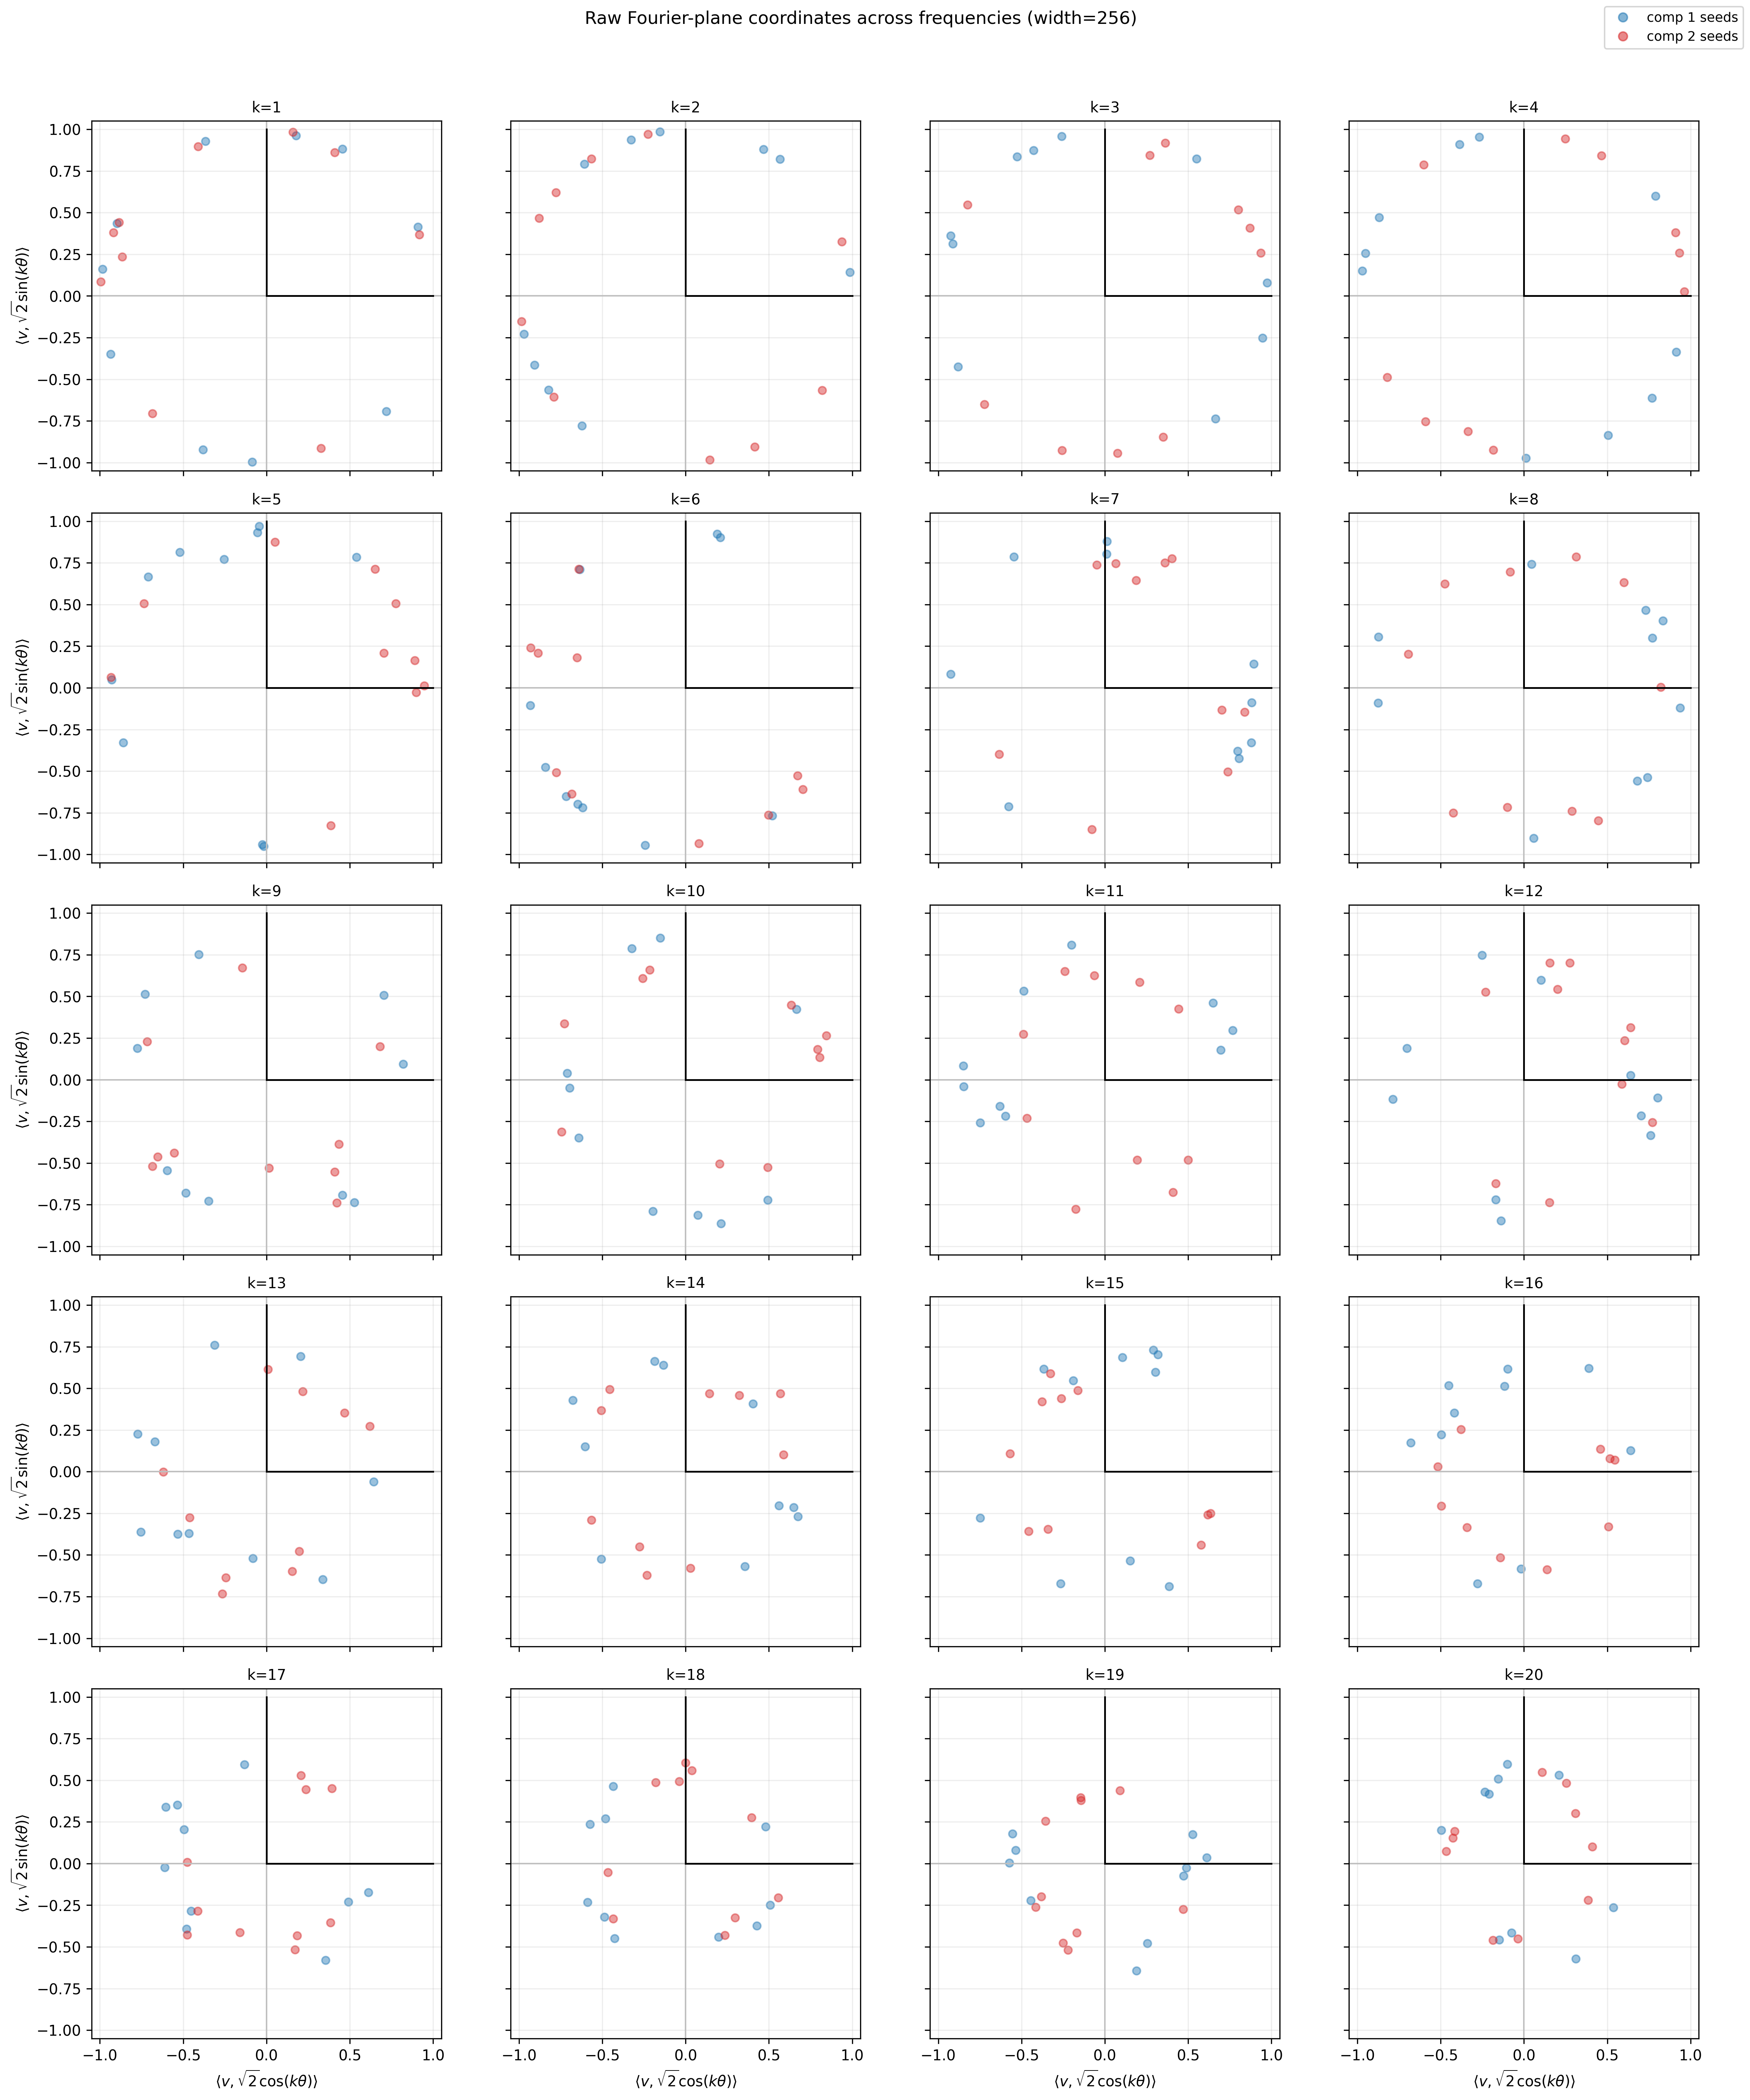
\includegraphics[width=0.92\textwidth]{images/ntk_eigenspace_alignment_on_S1/eigenvector_fourier_plane_raw_multi_freq_w256.png}
	\caption{Raw Fourier-plane coordinates across frequencies at width \(256\). For each \(k\), each seed contributes two points, one for each empirical component. Points near the unit circle indicate that the corresponding empirical eigenvector lies mostly inside the Fourier plane \(\mathcal F_k\); inward drift indicates leakage outside that plane. The lowest frequencies remain close to the circle, while higher frequencies become increasingly diffuse and contract toward the interior.}
	\label{fig:raw-fourier-plane-w256}
\end{figure}

\begin{figure}[H]
	\centering
	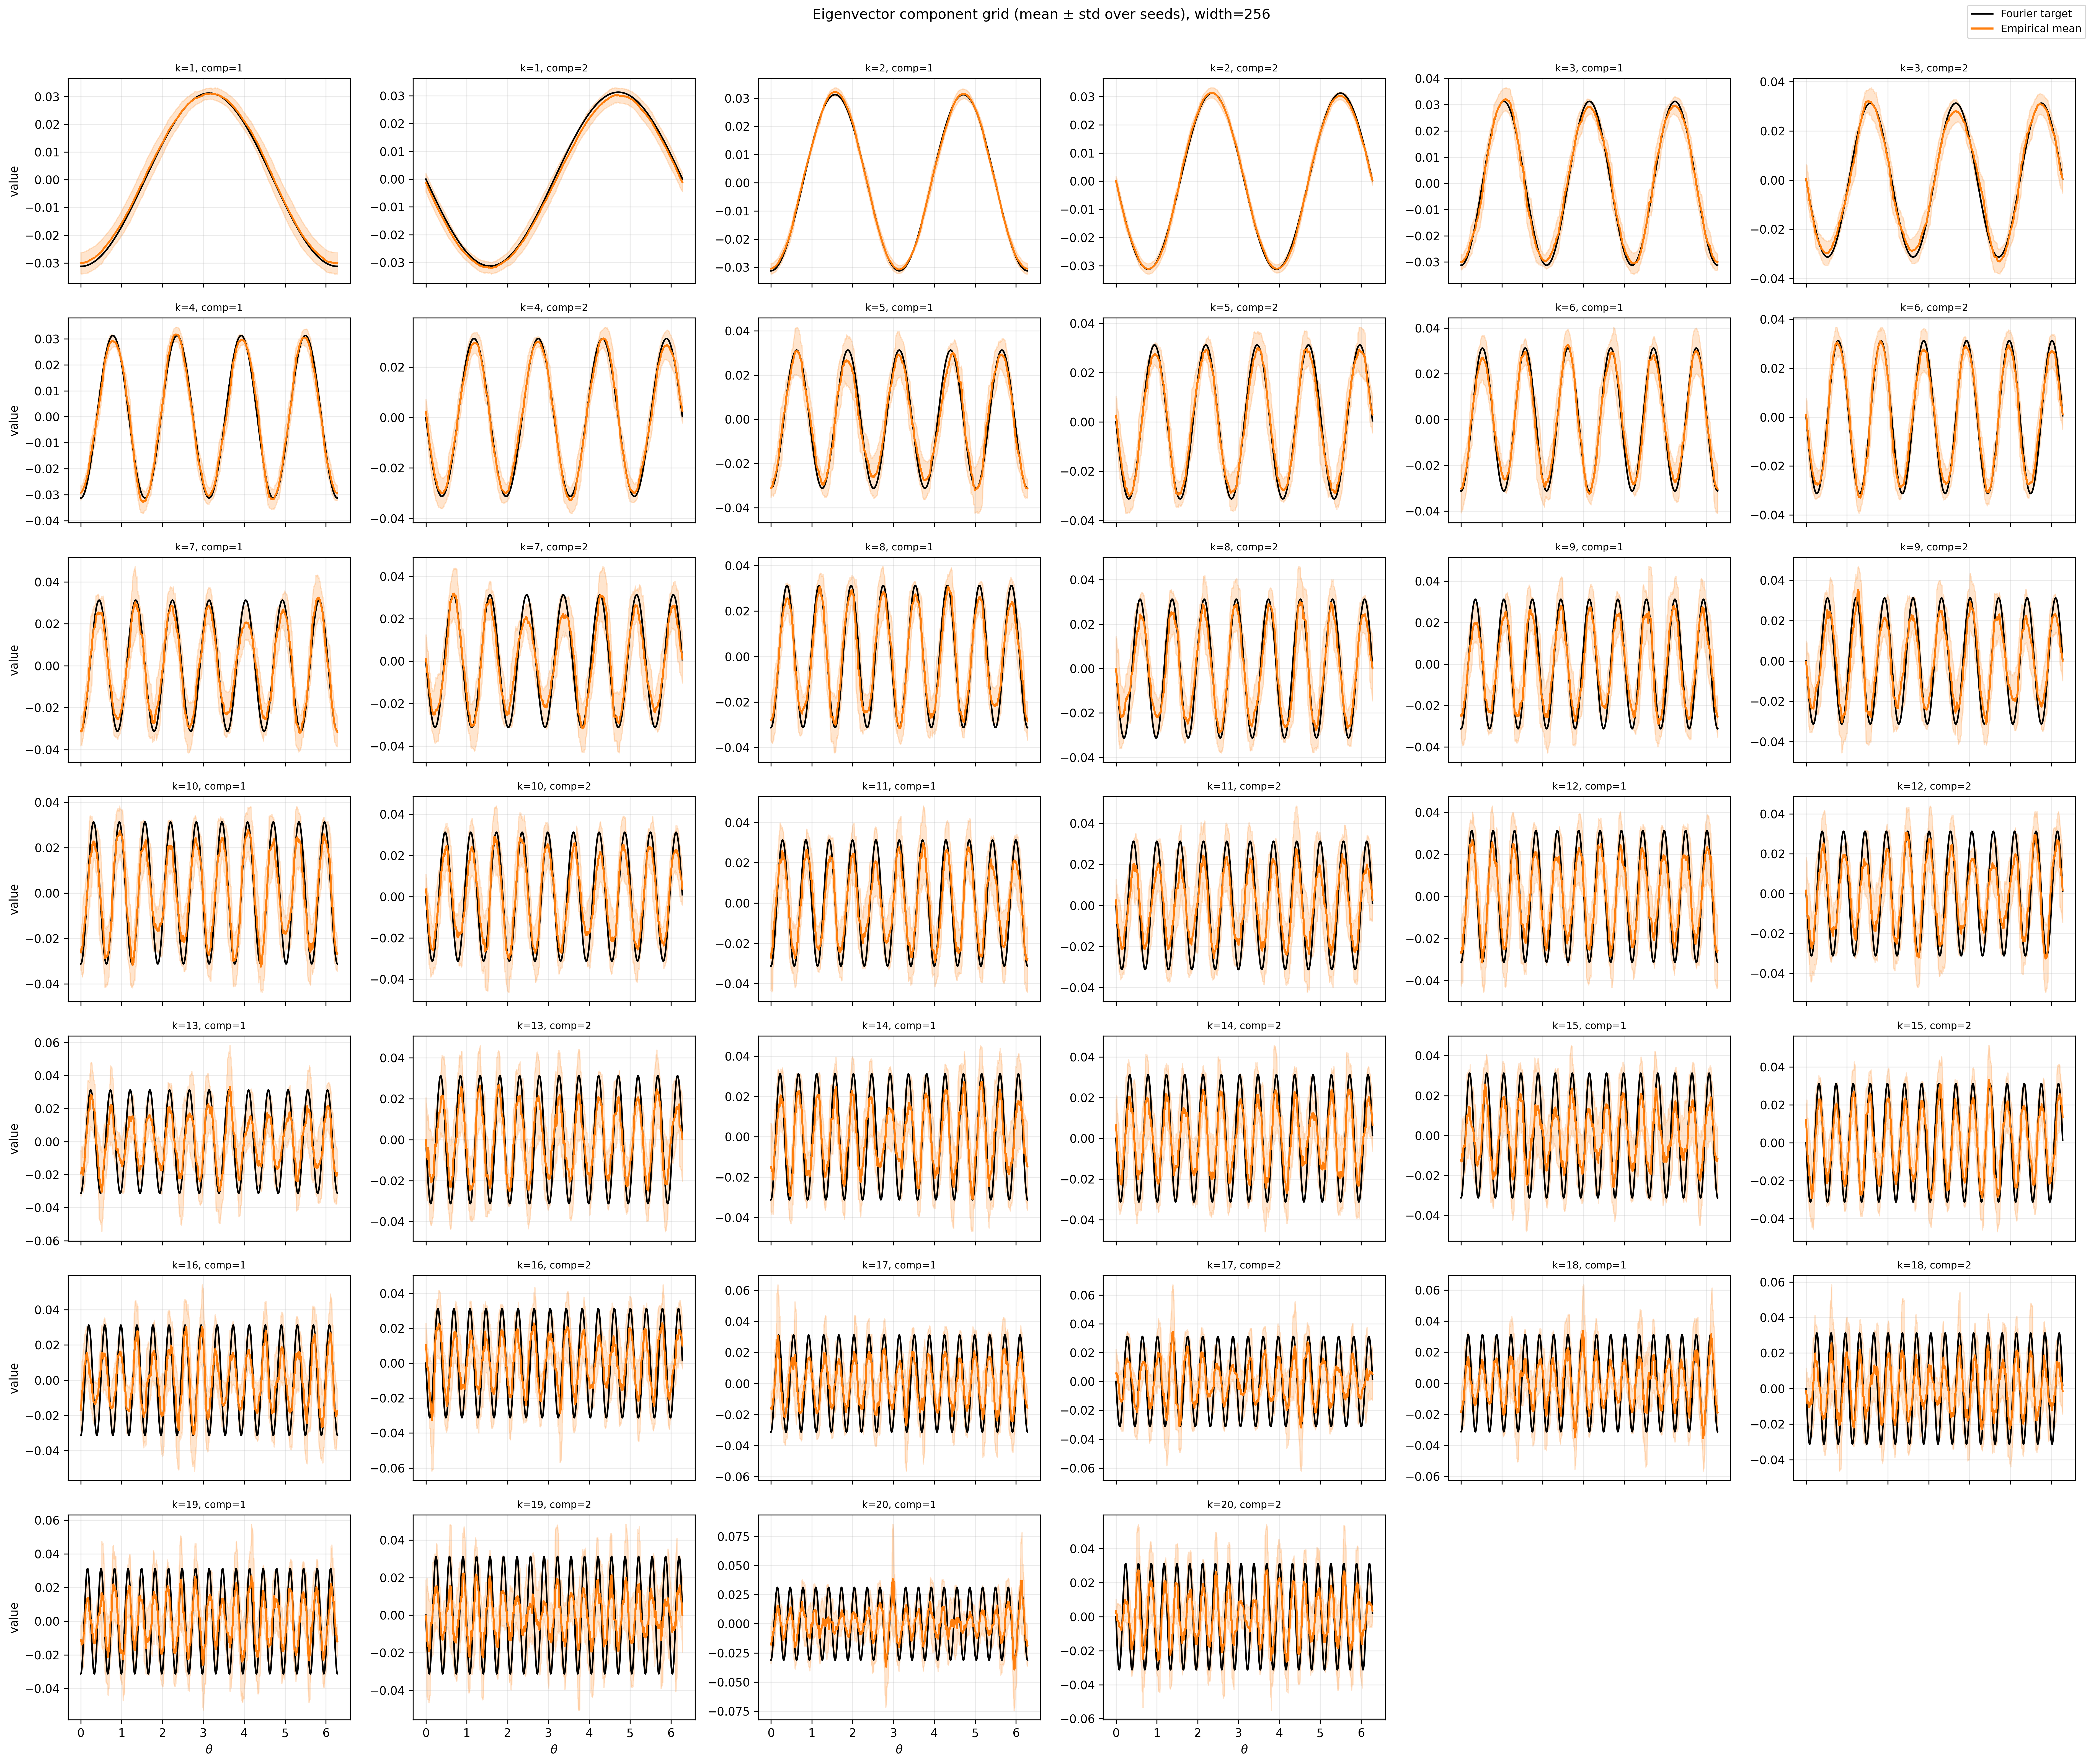
\includegraphics[width=0.92\textwidth]{images/ntk_eigenspace_alignment_on_S1/eigenvector_shape_grid_7x6_w256.png}
	\caption{Mean empirical eigenvector components (orange) versus the corresponding Fourier targets (black) at width \(256\), with shaded one-standard-deviation bands over seeds. The empirical components closely track the Fourier shapes at low frequencies, while phase and amplitude distortions, together with increased variability, become more pronounced as \(k\) increases.}
	\label{fig:eigenvector-shape-grid-w256}
\end{figure}

\begin{figure}[H]
	\centering
	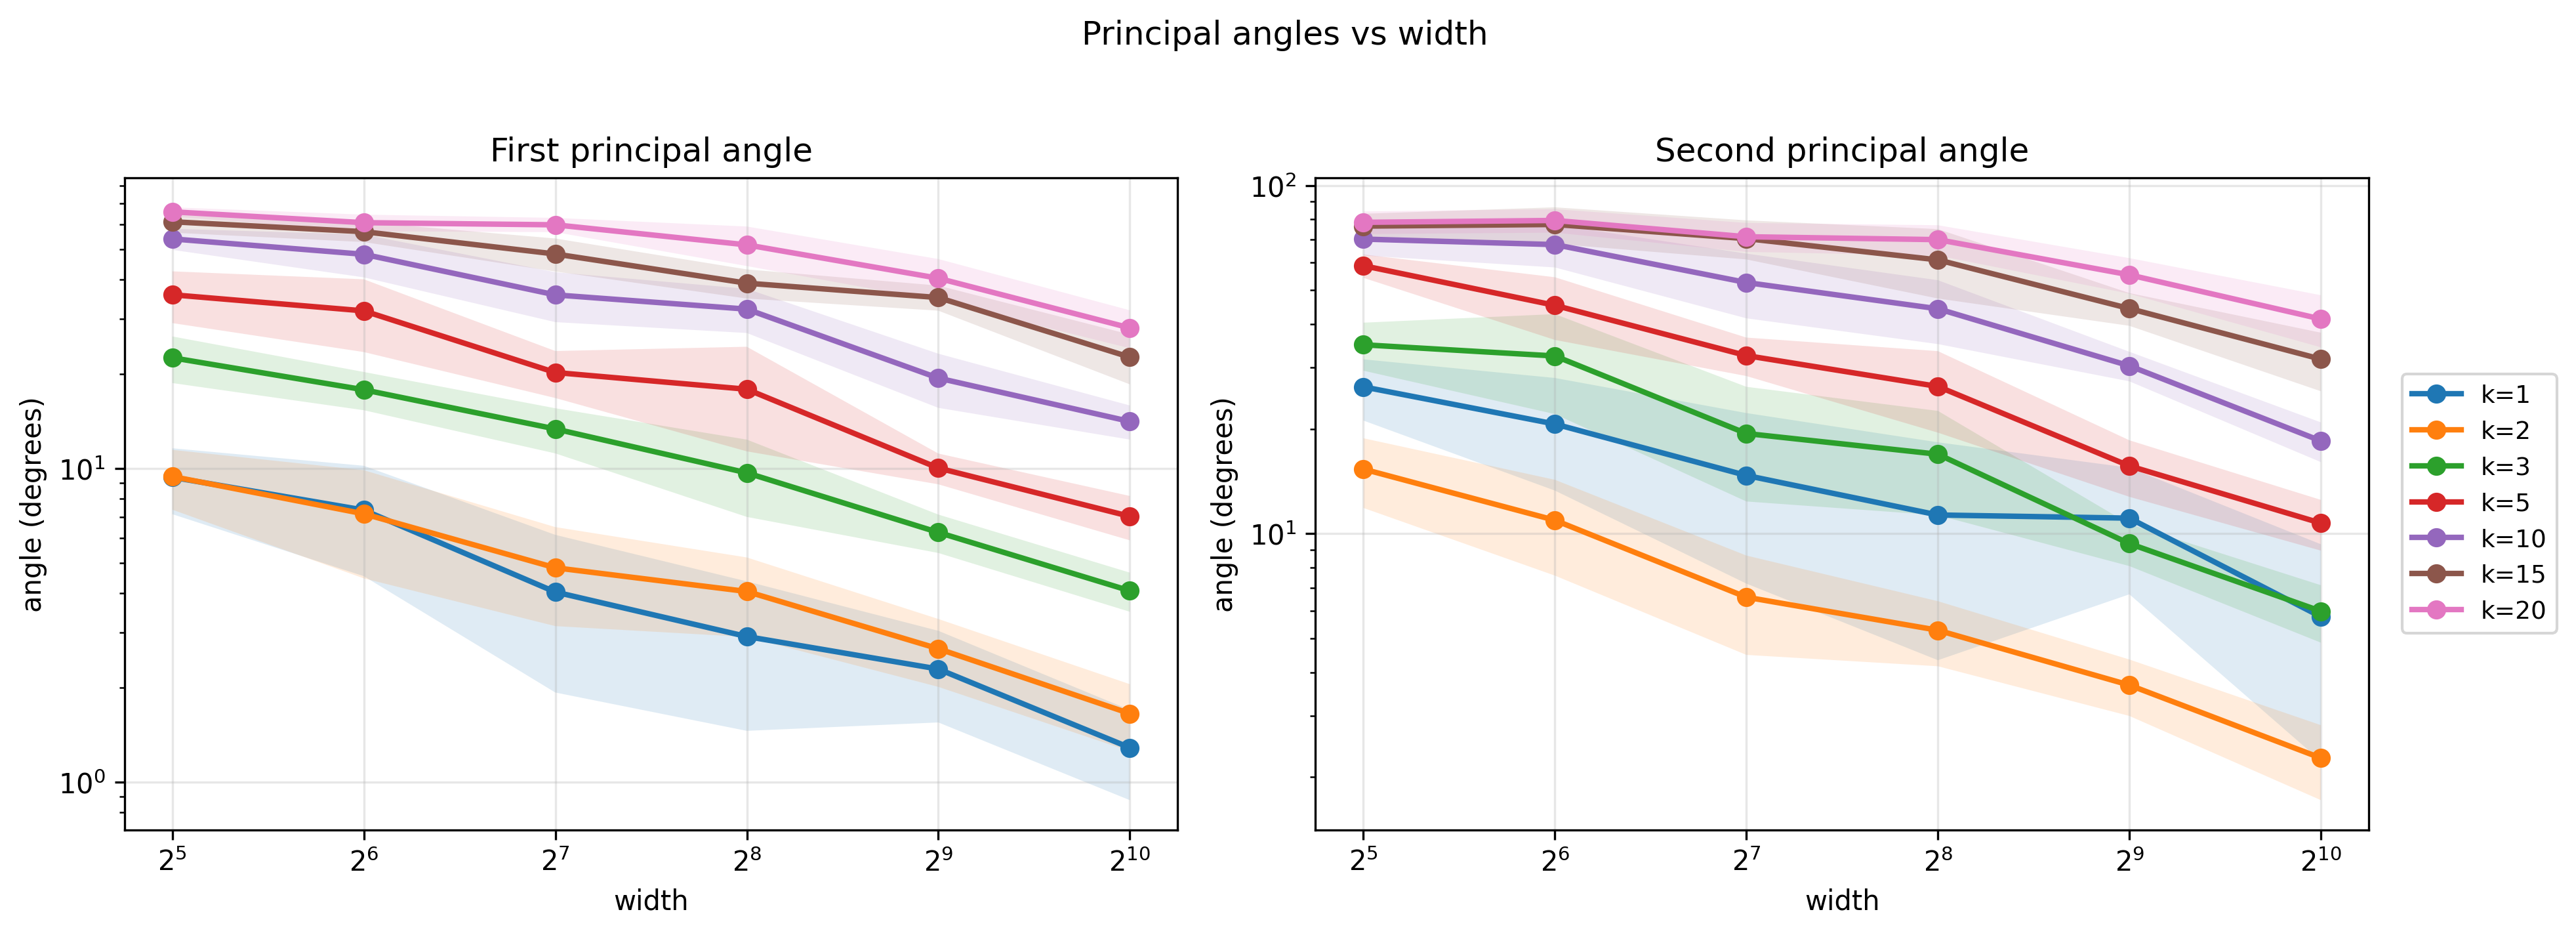
\includegraphics[width=0.92\textwidth]{images/ntk_eigenspace_alignment_on_S1/principal_angles_vs_width.png}
	\caption{Principal angles between the empirical frozen-kernel eigenspace and the corresponding Fourier plane, plotted against width for selected frequencies. Both angles decrease with width, but higher-frequency blocks align much more slowly. The second principal angle is crucial: it confirms whether the full two-dimensional Fourier subspace, and not just one preferred direction inside it, has been recovered.}
	\label{fig:principal-angles-vs-width}
\end{figure}

\begin{figure}[H]
	\centering
	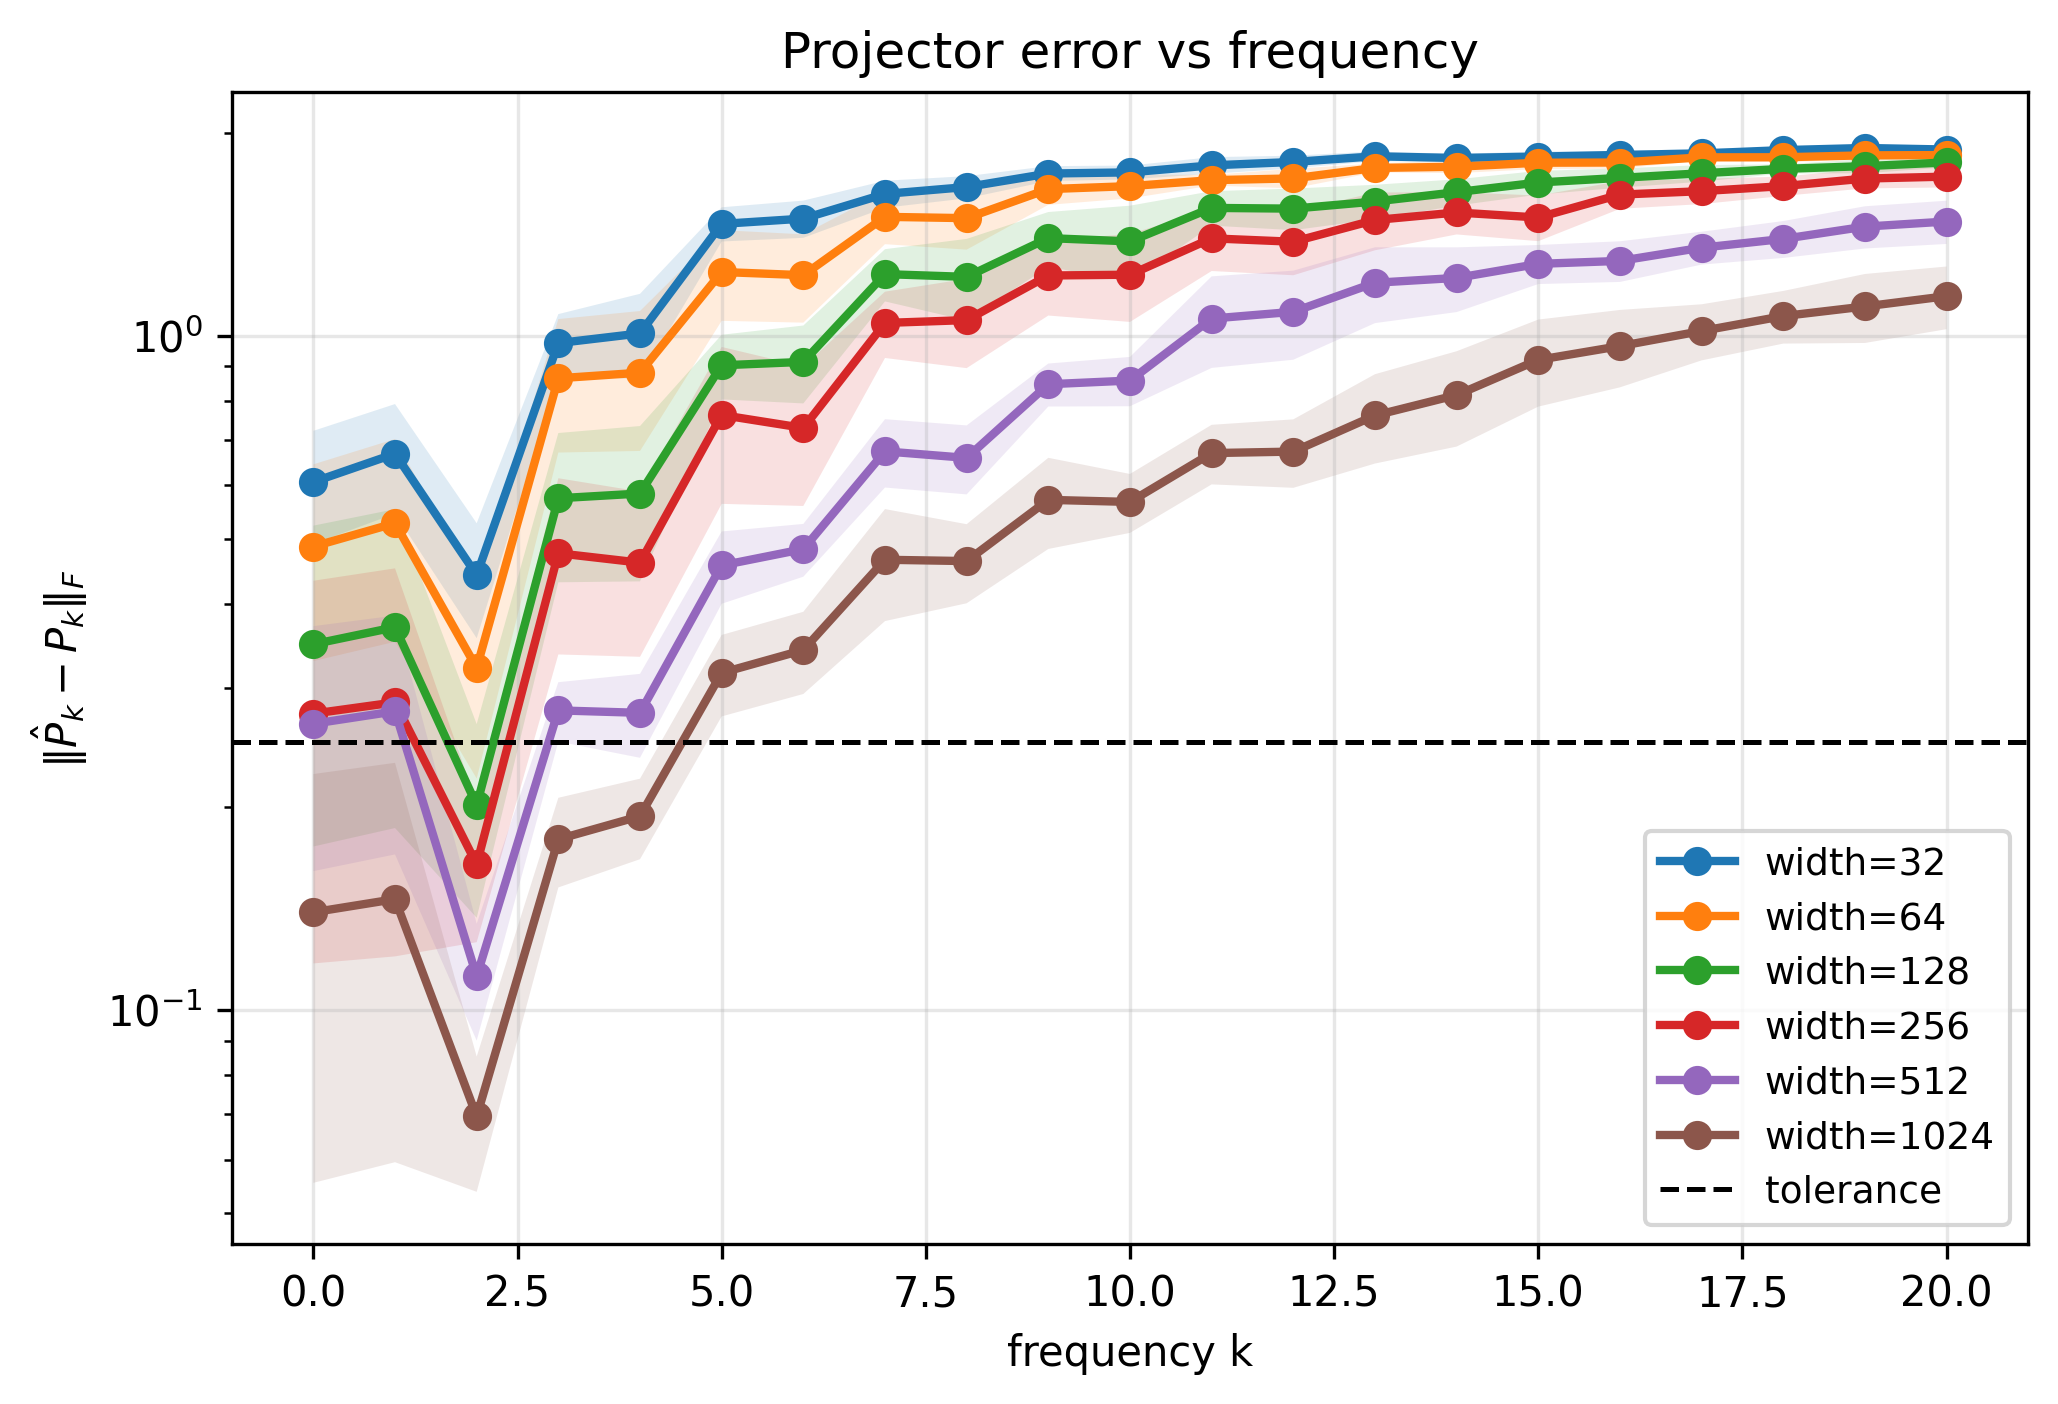
\includegraphics[width=0.92\textwidth]{images/ntk_eigenspace_alignment_on_S1/projector_error_vs_frequency.png}
	\caption{Projector error \(\|\widehat P_k-P_k\|_F\) as a function of frequency for different widths. The error grows rapidly with \(k\), showing that subspace recovery deteriorates significantly at higher frequencies even when the lowest modes are already well aligned.}
	\label{fig:projector-error-vs-frequency}
\end{figure}

\begin{figure}[H]
	\centering
	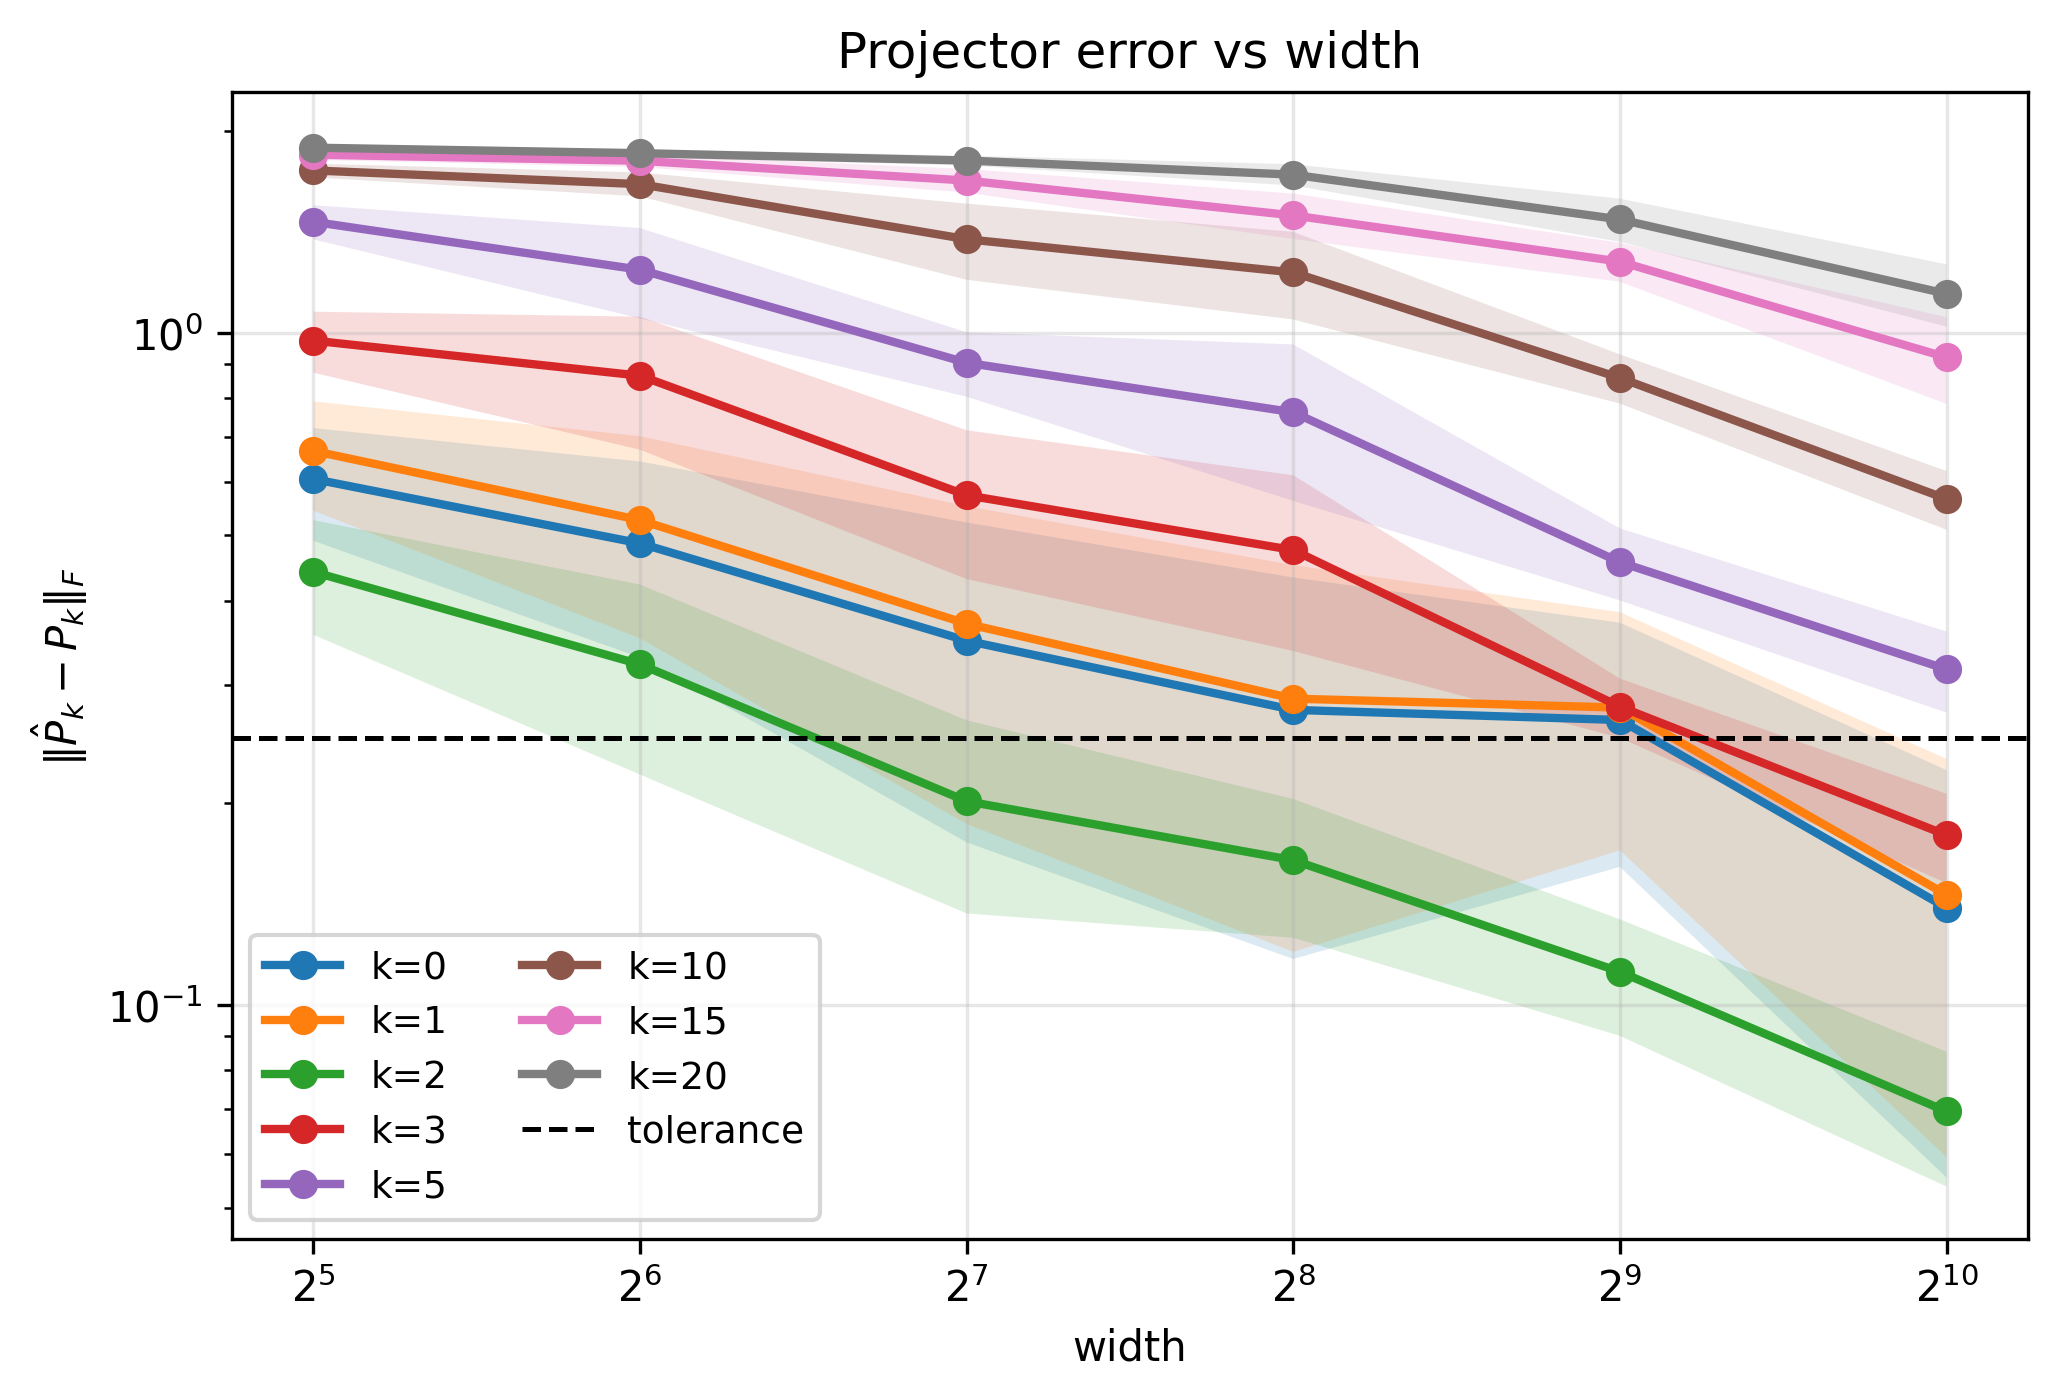
\includegraphics[width=0.92\textwidth]{images/ntk_eigenspace_alignment_on_S1/projector_error_vs_width.png}
	\caption{Projector error \(\|\widehat P_k-P_k\|_F\) as a function of width for selected frequencies. Alignment improves systematically with width, but only the lowest frequencies fall clearly below the tolerance threshold within the widths considered here.}
	\label{fig:projector-error-vs-width}
\end{figure}

\subsection{Frozen versus evolving NTK: mode dynamics and eigenspace drift at width \(256\)}
\label{subsec:frozen-vs-evolving-w256}

We now compare the frozen-kernel baseline with the fully evolving network at a fixed width \(m=256\), using the same initialization, target, and training data. In the notation above, the frozen branch keeps the compressed low-mode operator fixed at its initial value,
\[
	C_t^{(K)}\equiv C_0^{(K)},
\]
whereas the evolving branch uses the true time-dependent operator \(C_t^{(K)}\) generated by parameter training. The point of this comparison is to isolate the contribution of the operator-drift term
\[
	C_t^{(K)}-C_0^{(K)}
\]
in the projected dynamics
\[
	\dot u_t
	=
	-\Lambda_Ku_t
	-(C_0^{(K)}-\Lambda_K)u_t
	-(C_t^{(K)}-C_0^{(K)})u_t
	-\ell_t.
\]
If the frozen and evolving branches behaved similarly, then the initialization kernel would already explain most of the observed learning. If, instead, the evolving branch behaves differently and in particular fits better, then this difference must be attributed to the time-dependent deformation of the tangent operator and not merely to the frozen Fourier-diagonal baseline.

The training objective comparison shows that the evolving branch achieves a uniformly lower least-squares objective than the frozen branch throughout training and converges to a substantially smaller final loss. Thus, at width \(256\), the time dependence of the empirical NTK is not a negligible perturbation: allowing the kernel to evolve improves optimization in a measurable way.

To understand where this gain appears, we compare the residual projections onto selected Fourier modes. Across the displayed channels, the evolving branch is never worse asymptotically and is noticeably better on several of them. The improvement is especially clear for the constant mode and for the \(k=2\), \(k=5\), and \(k=6\) sine components, where the evolving branch reaches a visibly smaller residual amplitude than the frozen branch. For some channels, such as \(\cos_5\) and \(\cos_6\), the difference is more modest, but the evolving branch still tracks the frozen baseline closely and finishes at least slightly below it. The transient near-zero spikes visible on the logarithmic scale correspond to sign changes of the signed projection and should not be interpreted as abrupt loss of mode content. Overall, the mode trajectories show that the gain in objective value is accompanied by improved decay of several retained Fourier components, rather than by a uniform rescaling of all modes.

The principal-angle diagnostics show that this improved optimization is \emph{not} explained by the evolving kernel becoming more Fourier-aligned. In the frozen branch, the angles remain constant by construction. In the evolving branch, the angles increase almost immediately and then remain well above their frozen values. For \(k=2\), the drift is present but moderate: both principal angles rise above the frozen baseline and then slowly decrease, yet remain larger throughout training. For \(k=5\), the effect is much stronger: the first angle jumps from the frozen value of roughly \(16^\circ\) to the low \(40^\circ\) range, while the second angle rises from roughly \(25^\circ\) to the upper \(40^\circ\) range and stays there. For \(k=6\), the drift is even more pronounced, with the second angle spending most of training around \(60^\circ\) to \(70^\circ\). Thus, as the evolving network optimizes better than the frozen baseline, its empirical eigenspaces move \emph{away} from the corresponding Fourier planes rather than toward them.

The raw Fourier-plane coordinate grids corroborate this interpretation geometrically. The ``frozen'' and ``step \(0\)'' columns coincide, as expected. For \(k=2\), the evolving eigenspace remains relatively close to the Fourier circle and mainly undergoes a moderate in-plane rearrangement, consistent with the comparatively small increase in principal angles. By contrast, for \(k=5\) and especially \(k=6\), the evolving eigenspace contracts substantially inward and reorganizes away from the initial circle-like pattern. In the language of the raw coordinates, this means that the empirical eigenvectors retain less mass inside the Fourier plane and develop more leakage outside it. In the basis-free language of principal angles and projector errors, this means that the evolving eigenspaces are no longer well described by the corresponding frozen Fourier blocks.

Taken together, these plots show that the improvement of the evolving branch at width \(256\) does not come from remaining close to the frozen Fourier-diagonal structure. Rather, the opposite occurs: the evolving branch fits better \emph{while} its empirical eigenspaces drift away from the Fourier subspaces, especially at the harder frequencies \(k=5\) and \(k=6\). This is exactly the behavior predicted by the decomposition of the projected dynamics. The gain over the frozen baseline must therefore be attributed to the operator-drift term
\[
	-(C_t^{(K)}-C_0^{(K)})u_t,
\]
together with the accompanying changes in low-high coupling, and not to a more accurate preservation of the initial Fourier organization.

In other words, the frozen-kernel analysis provides a meaningful low-frequency baseline, but at width \(256\) the evolving network improves upon this baseline precisely by deforming the initial tangent operator in an optimization-relevant way. For the low modes that are already well aligned in the frozen experiment, such as \(k=2\), the deformation is modest but still beneficial. For more difficult modes such as \(k=5\) and \(k=6\), the deformation is substantial and accompanies the largest discrepancies between frozen and evolving behavior. This supports the interpretation that feature learning in the present setting should be understood not as better adherence to the frozen Fourier eigenspaces, but as a time-dependent reorganization of the tangent operator that changes effective rates, rotates eigenspaces, and improves optimization beyond what the frozen kernel alone can explain.

\begin{figure}[H]
	\centering
	
\includegraphics[width=0.9\textwidth]{images/ntk_frozen_vs_evolving_mode_dynamics_w256/train_ls_frozen_vs_evolving_w256.png}
	\caption{Least-squares objective comparison at width \(256\). The evolving branch achieves a uniformly lower training objective than the frozen NTK baseline and converges to a substantially smaller final loss, showing that kernel drift is optimization-relevant in this regime.}
	\label{fig:train-ls-frozen-vs-evolving-w256}
\end{figure}

\begin{figure}[H]
	\centering
	
\includegraphics[width=\textwidth]{images/ntk_frozen_vs_evolving_mode_dynamics_w256/mode_projection_trajectories_w256.png}
	\caption{Residual mode projections for selected Fourier channels at width \(256\). The evolving branch matches or improves upon the frozen baseline on all displayed modes and gives especially clear gains on the constant mode and on several sine components. The narrow dips to numerical zero on the logarithmic scale correspond to sign changes of the signed projection.}
	\label{fig:mode-projections-frozen-vs-evolving-w256}
\end{figure}

\begin{figure}[H]
	\centering
	
\includegraphics[width=\textwidth]{images/ntk_frozen_vs_evolving_mode_dynamics_w256/principal_angles_over_training_w256.png}
	\caption{Principal angles between the empirical eigenspaces and the corresponding Fourier planes during training at width \(256\). The frozen branch remains constant by construction. The evolving branch departs almost immediately from the frozen Fourier-aligned baseline, with the largest drift occurring for \(k=5\) and \(k=6\).}
	\label{fig:principal-angles-over-training-w256}
\end{figure}

\begin{figure}[H]
	\centering
	
\includegraphics[width=\textwidth]{images/ntk_frozen_vs_evolving_mode_dynamics_w256/raw_kernel_eigenspace_grid_frozen_vs_evolving_w256.png}
	\caption{Raw Fourier-plane coordinates of the empirical kernel eigenspaces for \(k=2,5,6\), comparing the frozen baseline with the evolving branch at several training steps. The frozen and step-\(0\) columns coincide. During training, the \(k=2\) eigenspace remains relatively close to the Fourier circle, whereas the \(k=5\) and \(k=6\) eigenspaces contract inward and reorganize away from the initial Fourier pattern, indicating increased leakage outside the corresponding Fourier planes.}
	\label{fig:raw-kernel-eigenspace-frozen-vs-evolving-w256}
\end{figure}

\end{document}
